\documentclass[aps,reprint]{revtex4-1}
% Engine-specific settings
% Detect pdftex/xetex/luatex, and load appropriate font packages.
% This is inspired by the approach in the iftex package.
% pdftex:
\ifx\pdfmatch\undefined
\else
    \usepackage[T1]{fontenc}
    \usepackage[utf8]{inputenc}
\fi
% xetex:
\ifx\XeTeXinterchartoks\undefined
\else
    \usepackage{fontspec}
    \defaultfontfeatures{Ligatures=TeX}
\fi
% luatex:
\ifx\directlua\undefined
\else
    \usepackage{fontspec}
\fi
% End engine-specific settings
\usepackage[english]{babel}
\usepackage{csquotes}
% \usepackage[backend=biber, sortcites]{biblatex}
\usepackage{url}
\usepackage{textcomp}
\usepackage[usenames,dvipsnames,svgnames, table]{xcolor}
\usepackage[font={scriptsize}]{caption}
\usepackage{amsmath} \usepackage{amsthm} \usepackage{amsfonts}
\usepackage{amssymb}
\usepackage{enumerate}
\usepackage{tikz}
\usetikzlibrary{backgrounds}
\usepackage{float}
\usepackage[procnames]{listings}
\usepackage{pstool} \usepackage{pgfplots}
\usepackage{wrapfig} \usepackage{graphicx} \usepackage{epstopdf}
\usepackage{afterpage}
\usepackage{physics}
\usepackage{multirow}
\usepackage{gensymb}
\usepackage{algorithm}
\usepackage{microtype}
\usepackage{algpseudocode}
\usepackage{xcolor,colortbl}
\usepackage{microtype}
\usepackage{geometry}
\usepackage{hyperref}
\usepackage{graphicx}
\usepackage{caption}
\usepackage{subcaption}
\usepackage{lipsum}
% \usepackage{pythontex}
% \usepackage{authblk}
\usepackage{nth}
\usepackage{siunitx}
% \usepackage[toc,page]{appendix}
\floatstyle{plaintop}
\restylefloat{table}

% Custom commands
\newcommand{\unit}[1]{\:\mathrm{#1}}
\newcommand{\noref}[1]{\hyperref[#1]{\ref*{#1}}}
\newcommand{\nonref}[1]{\hyperref[]{\ref*{#1}}}
\newcommand\blankpage{%
  \null
  \thispagestyle{empty}%
  \addtocounter{page}{-1}%
  \newpage}
\newcommand{\mean}[1]{\langle #1 \rangle}

% Default fixed font does not support bold face
\DeclareFixedFont{\ttb}{T1}{txtt}{bx}{n}{7} % for bold
\DeclareFixedFont{\ttm}{T1}{txtt}{m}{n}{7}  % for normal

\newcommand\numberthis{\addtocounter{equation}{1}\tag{\theequation}}
\DeclareCaptionFont{white}{\color{white}}
\DeclareCaptionFormat{listing}{\colorbox{gray}{\parbox{\columnwidth}{#1#2#3}}}
\pgfplotsset{compat=1.14} %TODO: Setting this removed several error messages, should it be here!?


% Biber for references
% \bibliographystyle{aipauth4-1}

\begin{document}
\sisetup{detect-all}
\title{Ising model for studies of phase transitions in magnetic systems - A computational approach}
\author{Frederik J. Mellbye}
\affiliation{University of Oslo, Oslo, Norway \\ Source code available at: \url{https://github.com/Caronthir/FYS3150/tree/master/Project4}}
\date{\today}

\begin{abstract}\noindent
The Ising model is investigated with a numerical implementation, and phase transitions
are found. Around $10^6$ Monte Carlo cycles are ran with the Metropolis
algorithm to perturb the spins for multiple lattice sizes, ranging from
2 to 100. For the $N = 2$ lattice size the method is shown to reproduce analytic
expectation values. The phase transition is found to occur at a critical temperature
within $T_C = 2.25 \pm 0.05$, which includes the analytical value $\approx 2.269$ by Onsanger.
The numerical value was not computed to a higher accuracy because of time
constraints and inconsistent susceptibility values.

\bigskip
\noindent \textbf{Disclaimer}:
\newline
For this project I collaborated with Erlend Lima with regards to the
analytic solutions presented, the code and therefore results and figures.
The text in this paper is written entirely by F. Mellbye, however there may be
several similarities with Lima's paper because the ideas and solutions
were discussed and developed together.
\end{abstract}
\maketitle
\tableofcontents
\makeatletter
\let\toc@pre\relax
\let\toc@post\relax
\makeatother

\newpage

\section{Introduction} \label{sec:introduction}
The Ising model, named after physicist Ernst Ising, is a widely used model for
ferromagnetism in statistical mechanics. The model is widely used in a wide range
of applications because it is the simplest model to exhibit phase transitions
in two dimensions. An analytic solution for the transition critical temperature
is available, as shown by Lars Onsager. Analytic solutions are also avalilable
for the one dimensional case.

A numerical solver is implemented which repeats a Metropolis algorithm scheme
in a series of Monte-Carlo cycles, which simulates the Ising model.
The system is simulated for larger and larger lattice sizes and thermodynamic
quantities such as heat capacity and magnetic susceptibility are found for
multiple temperatures. From these quantities the critical temperature for the
phase transition can be found.

In order to generalize the results the equations in this paper are scaled.
When no units are presented, energies and temperatures are scaled with $J$ and
$kT/J$, respectively. Because of the dimensionality of these quantities, the spins
and thus the system magnetic moment is dimensionless.
\section{Theory} \label{sec:theory}
\subsection{The Ising model}
A square lattice of $N \times N$ binary magnetic dipoles (quantified atomic spins)
make up the Ising model. The dipoles can only have spins $s_i$ up ($1$) and down ($-1$).
In the Ising model the temperature $T$ is held constant.

The energy is given by
\begin{align}\label{eq:energy}
  E = -J \sum_{\langle kl \rangle}^{N} s_k s_l
\end{align}
where for each lattice location the sum is taken over the neighbors only. $J$ is
a constant that determines the strength of the interaction between the nodes
(The complexity of the quantum mechanics in such a system is baked into
this constant). It is assumed that there is a ferromagnetic ordering so that $J > 0$.
There is also an additional term if an external magnetic field is applied, but
in this paper this is set to $0$.

The magnetization is simply given as the sum of the spins:
\begin{align}\label{eq:magmom}
  \mathcal{M} = \sum_i s_i
\end{align}

The thermodynamical quantities that are computed in this paper can be constructed
from the above expressions. The heat capacity under constant volume $C_V$ is given
by
\begin{align}\label{eq:Cv}
  C_V = \frac{\mean{E^2} - \mean{E}^2}{kT^2}
\end{align}
and the magnetic suceptibility is similarly given by
\begin{align}\label{eq:sus}
  \chi = \frac{\mean{\mathcal{M}^2} - \mean{\mathcal{M}}^2}{kT}
\end{align}
For a more extensive explaination and derivation of the above expressions see
\cite{mortenjensen}. Another equation which is also presented in the lecture notes
is a way to compute the expectation value of the energy $\mean{E}$:
\begin{align}\label{eq:meanE}
  \mean{E} = - \pdv{\ln{Z}}{\beta}
\end{align}

\subsection{Boundary conditions}
There are several ways to model the boundaries, which have different advantages
and disadvantages. Perhaps the easiest solution is for the boundary spins to have
no outside neighbors. Usually real materials have an enormous amount of spins,
and the effect of the boundaries is negligible. In the Ising model an infinite
number of spins is not possible, and for small lattice sizes an appropriate
method needs to be used. For the intents and purposes of this paper, an ideal
method is to have so-called periodic boundaries. This involves treating the
spins on the oppsite side of the lattice as the neighbors of the boundary spins.
This is a much better approximation to an infinitely large lattice, because
each spin has access to four neighbors.

\subsection{Metropolis algorithm} \label{sec:theory_metro}
Monte-Carlo simulations are used to model the time development of the system.
With some initial configuration, an algorithm that over time modifies the system
to an equilibrium state needs to be employed. A method which has been shown to
do this is the famous Metropolis algorithm. See chapter .. in CITE for a detailed explaination
of the algorithm, the main steps are as follows:
\begin{enumerate}
  \item Select randomly $N^2$ spins in the lattice.
  \item Calculate the system change in energy $\Delta E$ if a randomly selected spin was to
  be flipped.
  \item Draw a random number from the uniform distribution, and compare
  \begin{align*}
    U(0,1) \leq e^{-\beta \Delta E}.
  \end{align*}
  If this is true, the spin is flipped. If this evaluates as false, do not flip
  the spin. If $\Delta E < 0$ the spin is flipped regardless, to model that physical
  systems usually tend to lower energy configurations.
\end{enumerate}
When this is repeated multiple times the system will converge to the equilibrium
state. In this model, the system development with Monte-Carlo cycles can therefore be
considered the system development with time. The comparison of the random number
is with boltzmann factors, which therefore completely shape the system behaviour.
Because these factors are functions of temperature, the system flip behaviour is
expected to change perhaps drastically with temperature.
\subsection{Phase transitions in the Ising model} \label{sec:phase transitions analytic}
One of the properties of the Ising model is that phase transitions can be
observed. The transition occurs at a critical temperature $T = T_C$, where
the spins fluctuate at a maximum rate. The rapid fluctuations result in high
variances in energy and magnetic moment, i.e. a maximum for the heat capacity
and susceptibility. According to \cite{project4} these quantities can be
modelled as
\begin{align*}
  \mean{M(T)} &\sim (T - T_C)^\beta \\
  C_V(T) &\sim |T_C - T|^\gamma \\
  \chi (T) &\sim |T_C - T|^{-\alpha}
\end{align*}
where $\alpha = 0$, $\beta = 1/8$ and $\gamma = 7/4$ are critical exponents.
The critical temperature is ideally computed for an infinite lattice size. Therefore
our finite sized lattice will only be an approximation, however, luckily there is
a connection between the finite and infinite lattice values. According to
\cite{project4}:
\begin{align}\label{eq:crit_relation}
  T_C(L) - T_C(L = \infty) = a L^{-1/\nu}
\end{align}
where $\nu$ is found using equation 2 in \cite{project4}. The exact result for
this value is $\nu = 1$. $a$ is a constant, which can be determined by comparing
the critical temperatures for two different lattice sizes:
\begin{align}\label{eq:scalingfactor}
  a = \frac{T_C(L_1) - T_C(L_2)}{L_1^{-1/\nu} - L_2{-1/\nu}}
\end{align}
When the scaling factor $a$ is found, this can be inserted in equation~\ref{eq:crit_relation}
to find the infinite lattice value.
\subsection{Analytic solution in the 2 x 2 lattice case}
For the simple case of a $2 \times 2$ periodic boundary lattice analytic
expressions can be computed, which will be used to check that the numerical
implementation produces acceptable results. The four spins are enumerated as in
figure~\ref{fig:22lattice}.
\begin{figure}
  \centering
  \begin{tikzpicture}[thick]
    \draw[->] (0,0) -- (0,.3)  node [label=left:{$s_1$}] {};
    \draw[->] (1,0) -- (1,.3)  node [label=right:{$s_2$}] {};
    \draw[->] (0,1) -- (0,1.3) node [label=left:{$s_3$}] {};
    \draw[->] (1,1) -- (1,1.3) node [label=right:{$s_4$}] {};
    \draw[dotted] (-.75,-.4) rectangle (1.75,1.9);
  \end{tikzpicture}
  \caption{$2 \times 2$ enumerated lattice with all spins pointing up.}
  \label{fig:22lattice}
\end{figure}
A short walkthrough and the relevant equations are presented here, the equations
and derivations are entirely based on \cite{mortenjensen}. In a $2 \times 2$
lattice, there are $2^4 = 16$ possible microstates (unique configurations). Each
microstate is associated with thermodynamical quantities, such as energy and
magnetization, which determines the partition function. From this it is possible
to derive multiple statistical properties of the system.

Energies and magnetizations for the different possible configurations were calculated
using the method presented in the lecture notes by Hjort-Jensen.
The results of the calculations are shown in table~\ref{tab:2x2values}.

\begin{table}[H]
  \caption{Possible states and associated energies, magnetizations and degeneracies.
  The same table is also found in \cite{mortenjensen}}
  \label{tab:2x2values}
  \begin{ruledtabular}
    \begin{tabular}{cccc}
      Spins up & Energy [$J$] & Magnetization & Multiplicity \\
      4        & -8           & 4             & 1            \\
      3        & 0            & 2             & 4            \\
      2        & 0            & 0             & 4            \\
      2        & 8            & 0             & 2            \\
      1        & 0            & -2            & 4            \\
      0        & -8           & 4             & 1
    \end{tabular}
  \end{ruledtabular}
\end{table}
With the entries in the above table it is possible to calculate the partition
function, which is given by
\begin{align} \label{eq:partitionfunc}
  Z = \sum_i e^{\beta E_i}
\end{align}
where $\beta = 1/kT$. By simply summing over all the microstates with equation~\ref{eq:partitionfunc}
one finds
\begin{align*}
  Z = 2 e^{8\beta J} + 2 e^{- 8\beta J} + 12 = 4 \cosh{(8\beta J)} + 12
\end{align*}
When the partition function is known, the statistical thermodynamical quantities
of interest can be computed. To save space the algebra steps are omitted,
and the relevant expressions are listed here:

The mean energy (energy expectation value) is given by
\begin{align*}
  \mean{E} = -\frac{8 J \sinh{(8\beta J)}}{\cosh{(8\beta J)} + 3}
\end{align*}
and the mean of the square of the energy is given by
\begin{align*}
  \mean{E^2} = \frac{256 J^2 \cosh{(8\beta J)}}{4\cosh{8\beta J} + 12}.
\end{align*}
The energy expressions can be used to compute the heat capacity $C_V$, which
is given by
\begin{align*}
  C_V = \frac{1}{kT} \left( \mean{E^2} - \mean{E}^2 \right)
\end{align*}

Similarly, the magnetization properties are given by
\begin{align*}
  \mean{M} &= 0 \\
  \mean{M^2} &= \frac{8e^{8 J \beta} + 8}{\cosh{8\beta J} + 3}
\end{align*}
which can be used to find the susceptibility using equation~\ref{eq:sus}.

The general method to find the $n$-th moment of some quantity $A$ that was
used is:
\begin{align*}
  \mean{A^n} = \frac{1}{Z} \sum_i^{16} A_i^n e^{-\beta E_i}
\end{align*}

\section{Method} \label{sec:method}
All of the numerical calculations were done in C++, and the results were analyzed
with Python. See the attatched Github repository for more information about code workflow.
The project has extensive unit testing using the library Google Test. The lattice time
development was also animated, an example of this is also available on GitHub.
\subsection{Implementing the Metropolis algorithm}
The entire code is outlined in algorithm~\ref{algo:Metropolis}.
\begin{algorithm}[H]
  \caption{Monte Carlo and Metropolis algos outline.}
  \label{algo:Metropolis}
   \begin{algorithmic}[1]
     \For{$T$ in Selected Temperatures}
        \State Reset expectation value variables
        \State Initialize $E = -\sum_{\mean{k,l}}s_k s_l$, $M = \sum_i s_i$
        \For{$i = 1,2,\hdots, M$ (MC cycles)}
          \For{$j = 1,2,\hdots, N$ (Lattice)}
            \State Draw random $s_{m,n}$, calculate d$E$.
            \State Metropolis: Accept/reject (~\ref{sec:theory_metro})
            \State Update $s_i$'s, $E$ and $\mathcal M$ if accepted
          \EndFor
        \EndFor
        \State Calculate expectation values. Save.
     \EndFor
   \end{algorithmic}
\end{algorithm}
The algorithm essentialy simulates a battle between the tendency of physical systems
to fall to lower energy states and other physical effects such as thermal
effects which randomly add energy. This rather simple model surprisingly
reproduces several effects such as phase transitions. This is presented further in
~\ref{sec:phase transitions}.

\subsection{Energy calculations}
Calculating the total energy of the system is a quite time consuming task, having
to sum all four neighbors of each member of the lattice for each MC cycle. Fortunately,
this is not neccesary, because when a spin is flipped, the system change in energy
only depends on the four neighbors. There is only a limited amount of possible
such configurations, and thus a limited amount of possible energy changes. These
can therefore be precomputed. As seen in \cite{mortenjensen}, the possible
energy changes $\Delta E$ are $-8, -4, 0, 4, 8$ (in units of $J$).

The boltzmann factors can therefore be precomputed, and simply called when a $\Delta E$
is proposed. Because only changes in energy are calculated when the MC-cycles
are running, the initial total energy is computed before the loop is initiated.
The implementation is available in the source code.
\subsection{Periodic boundaries}
In this paper, the boundaries are set periodic to mimic real-world behaviour and
thus acheive better results. A clever method was used to implement this, which
involves utilizing modulo division. In c++ arrays of length $N$ are indexed from
$0$ up to, and including $N-1$, so the expression
\begin{align*}
  i_\text{checked} = (i + N) \% N
\end{align*}
should return opposite index when the boundaries are crossed, and the same
index when inside the boundaries. We see that if $i \in [0, N-1]$ then $i$
remains unchanged, which is what we want. If $i = N$ (outside the upper boundary),
then the returned $i$ will be converted to $0$, which is the next element for
periodic boundaries. Also, if the lower boundary is crossed, i.e $i = -1$, then
the expression returns $N - 1$, exactly what is expected of the function.

\subsection{Time taken to reach equilibrium}
The square lattice is extended to have $N = 20$ spins in each direction. By simply
plotting some expectation values against the number of Monte Carlo cycles (which
is equivalent with time in our model) it is possible to make a rough estimate
for the equilibrium time of the system. This analysis is done with ordered
(all spins pointing in the same direction) initial states, and random
spin orientations, and repeated for different temperatures.

Another interesting quantity to investigate is the number of accepted flips as
a function of Monte Carlo cycles for different temperatures. Lower amounts of
accepted flips indicates that the system is not changing much, which is a strong
indication for whether the system is in equilibrium.
\subsection{Phase transitions} \label{sec:phase transitions}
To find the critical temperature for the Phase transition in the Ising model
the lattice size is increased gradually to $N = 100$. The analytic result in
\cite{onsager} states that $T_C \approx 2.269$, so the investigation is done
for temperatures close to this value. It is expected that the as the lattice size
increases the approximation should improve, and the critical temperature should
therefore approach the analytical value by Onsager.

The heat capacity is plotted against temperature for temperatures around the
analytical value, and the temperature for which the heat capacity (proportional
to the energy variance) is at a maximum is the critical temperature. This result
is compared to the equations in section~\ref{sec:phase transitions analytic}.

\subsection{Probability distribution}
The probability of the system having a certain energy $P(E)$ is conputed
for a system with a lattice size $N = 20$ at temperatures $T = 1$ and $T = 2.4$.
The method is simple, the amount of times a certain energy appears is counted
and stored in bins. This is compared with the computed variance in energy.

\subsection{Parallelization}
The code was also parallelized with MPI. This simply increases the amount of
data produced by approximately a factor of the number of processors available,
which yields higher quality results in the same time.

\subsection{Random number generator}
The famous Mersenne Twister PRNG was used for all the random number generation
in the code. The very long period of $2^{19937} - 1$ and fast number generation
compared to other RNGs were the main reasons for this choice.
\section{Results} \label{sec:results}
All of the values and figures presented in the results are per spin and Monte Carlo
iteration, in order to have as general results as possible.
\subsection{$2 \times 2$ lattice. Comparison of numerical and analytical values.}
Figures~\ref{fig:L2Ne4},~\ref{fig:L2Ne5} and~\ref{fig:L2Ne6} show
the heat capacity for $T = 1$ and different amounts of MC cycles.
\begin{figure}
  \centering
  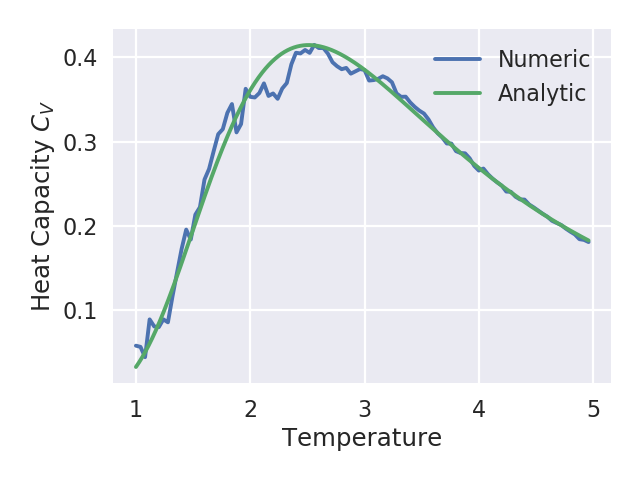
\includegraphics[width=\columnwidth]{figures/L2Ne4.png}
  \caption{$2 \times 2$ lattice with $M = 10^4$ MC iterations.}
  \label{fig:L2Ne4}
\end{figure}
\begin{figure}
  \centering
  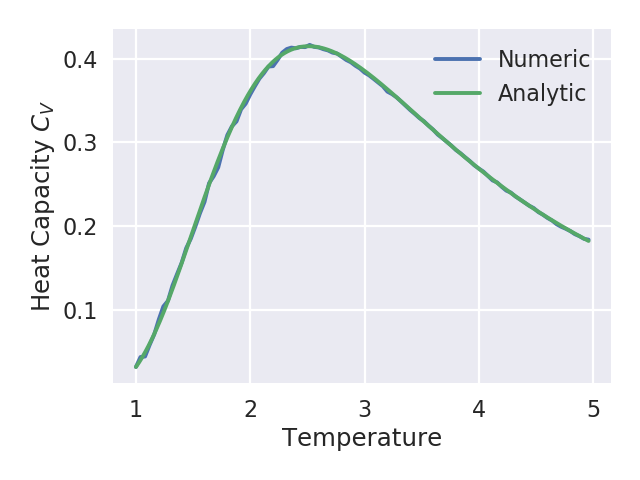
\includegraphics[width=\columnwidth]{figures/L2Ne5.png}
  \caption{$2 \times 2$ lattice with $M = 10^5$ MC iterations.}
  \label{fig:L2Ne5}
\end{figure}
\begin{figure}
  \centering
  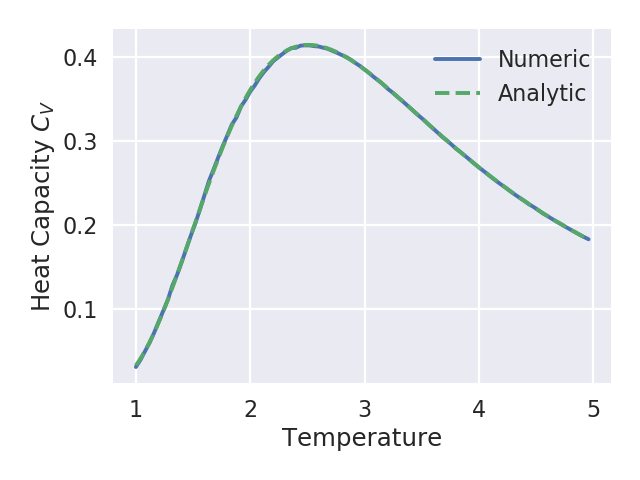
\includegraphics[width=\columnwidth]{figures/L2Ne6.png}
  \caption{$2 \times 2$ lattice with $M = 10^6$ MC iterations.}
  \label{fig:L2Ne6}
\end{figure}
Figure~\ref{fig:animals} shows several thermodynamic expectation values
as a function of temperature for a sufficient amount of Monte Carlo iterations.
\begin{figure}
  \begin{tabular}{cc}
    \centering
    \begin{subfigure}[b]{0.5\columnwidth}
        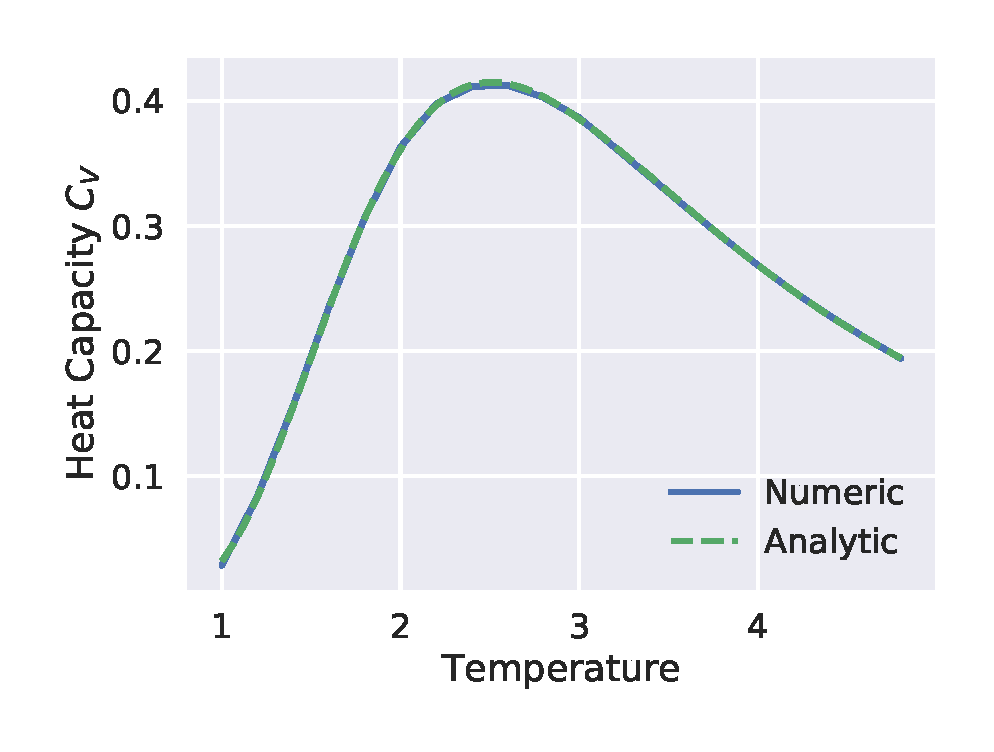
\includegraphics[width=\columnwidth]{figures/4bHeatCapacity.eps}
        \caption{Heat Capacity}
        \label{fix1}
    \end{subfigure}&
    \begin{subfigure}[b]{0.5\columnwidth}
        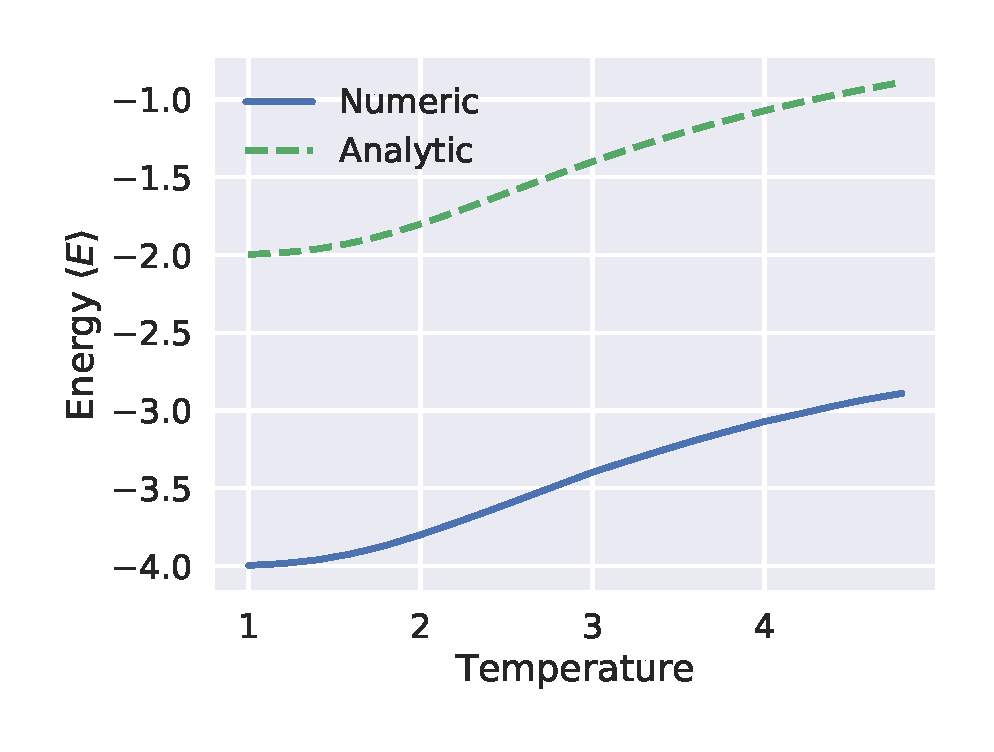
\includegraphics[width=\columnwidth]{figures/4bEnergy.eps}
        \caption{Energy}
        \label{free1}
    \end{subfigure}\\
    \begin{subfigure}[b]{0.5\columnwidth}
      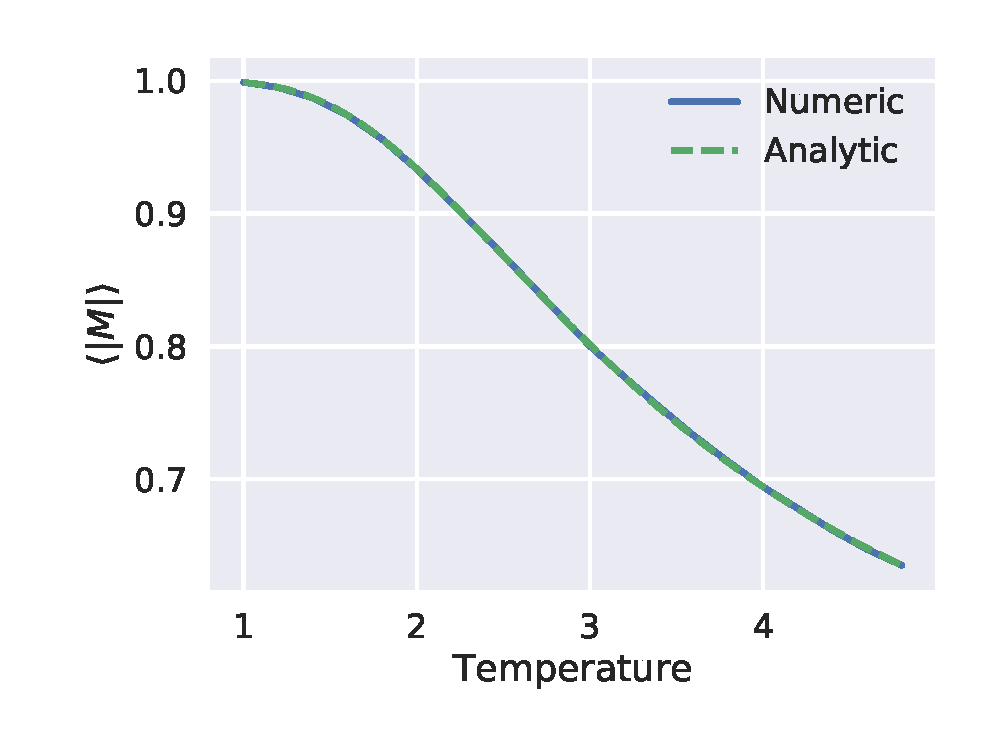
\includegraphics[width=\columnwidth]{figures/4bMagnetization.eps}
        \caption{Magnetization}
        \label{fix10}
    \end{subfigure}&
    \begin{subfigure}[b]{0.5\columnwidth}
        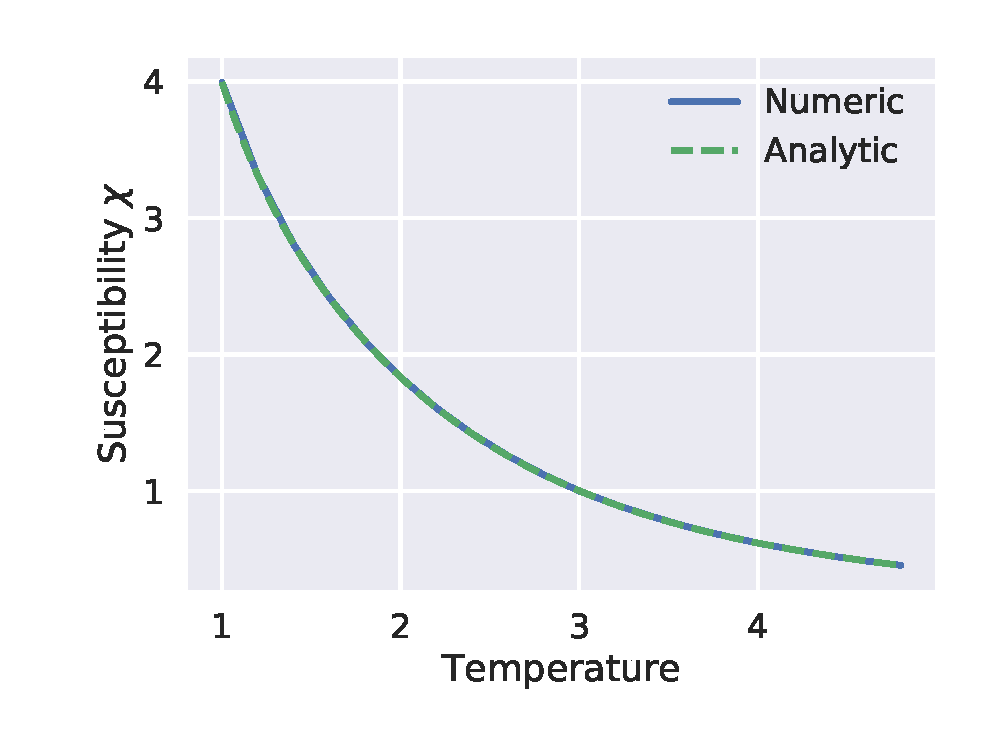
\includegraphics[width=\columnwidth]{figures/4bSusceptibility.eps}
        \caption{Susceptibility}
        \label{free10}
    \end{subfigure}\\
    \end{tabular}
    \caption{$2 \times 2$ lattice simulation results with $M = 10^6$ MC cycles
    for each temperature.}
    \label{fig:animals}
\end{figure}

\subsection{Time taken to reach equilibrium}
Figures~\ref{fig:L20T1Random} and~\ref{fig:L20T24Random} show the energy,
magnetization and spin flip time development for different temperatures.
\begin{figure}
  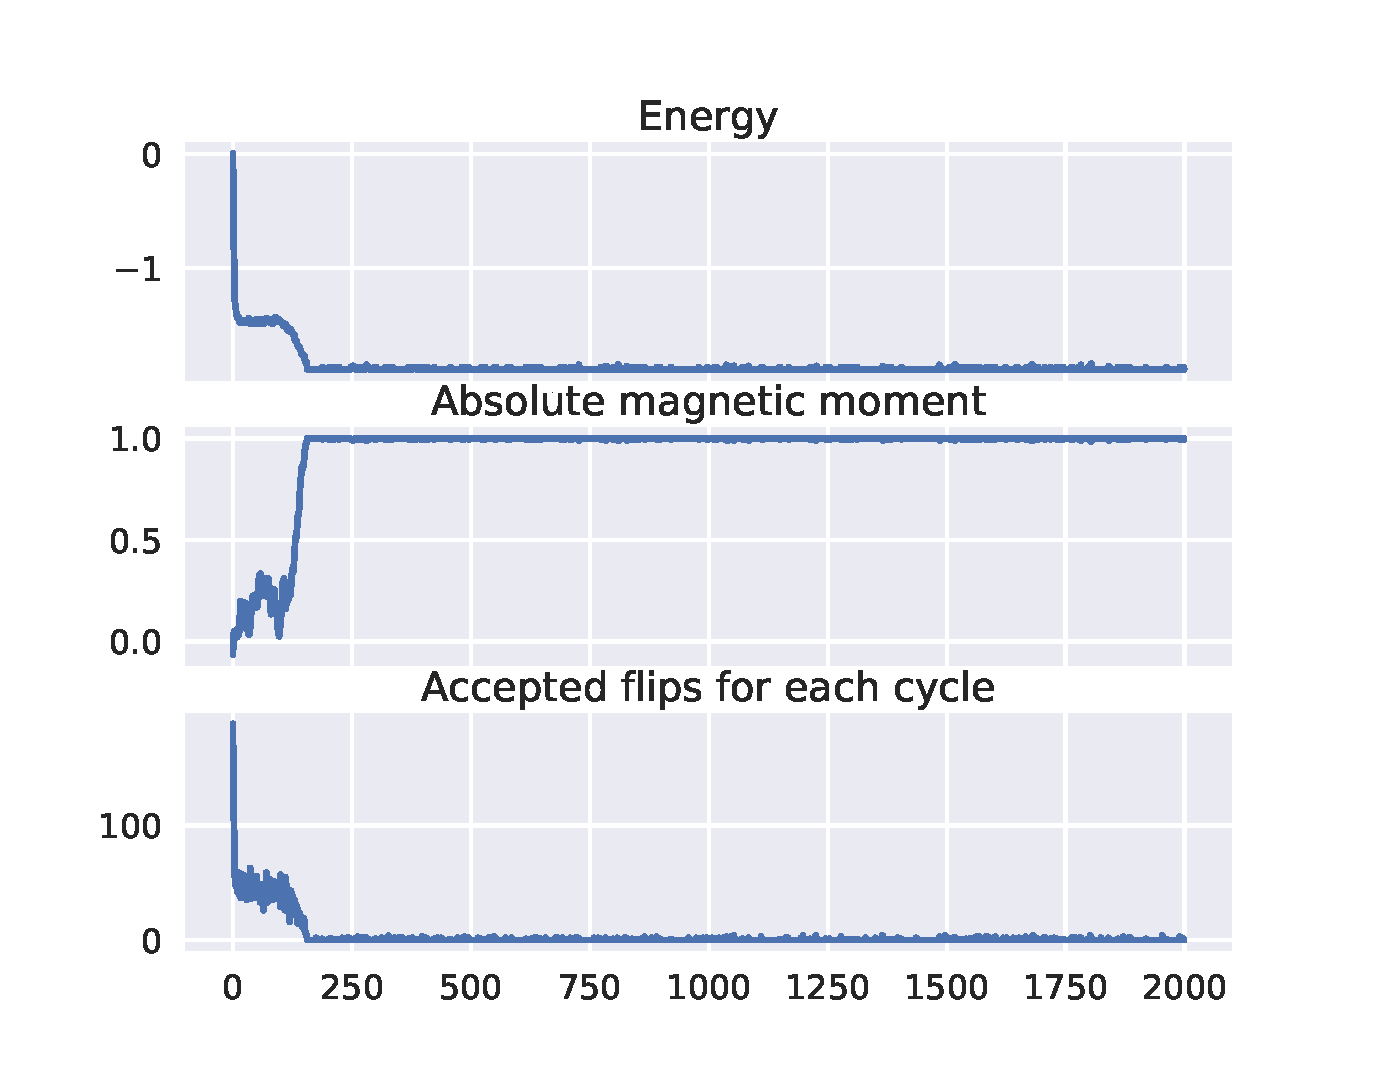
\includegraphics[width=\columnwidth]{figures/L20T1_random.eps}
  \caption{Energy, absolute magnetization and number of flips as a function of
  Monte Carlo cycles. The lattice size is $N = 20$, and the temperature $T = 1$ kT/J.
  The initial configuration is randomized.}
  \label{fig:L20T1Random}
\end{figure}
\begin{figure}
  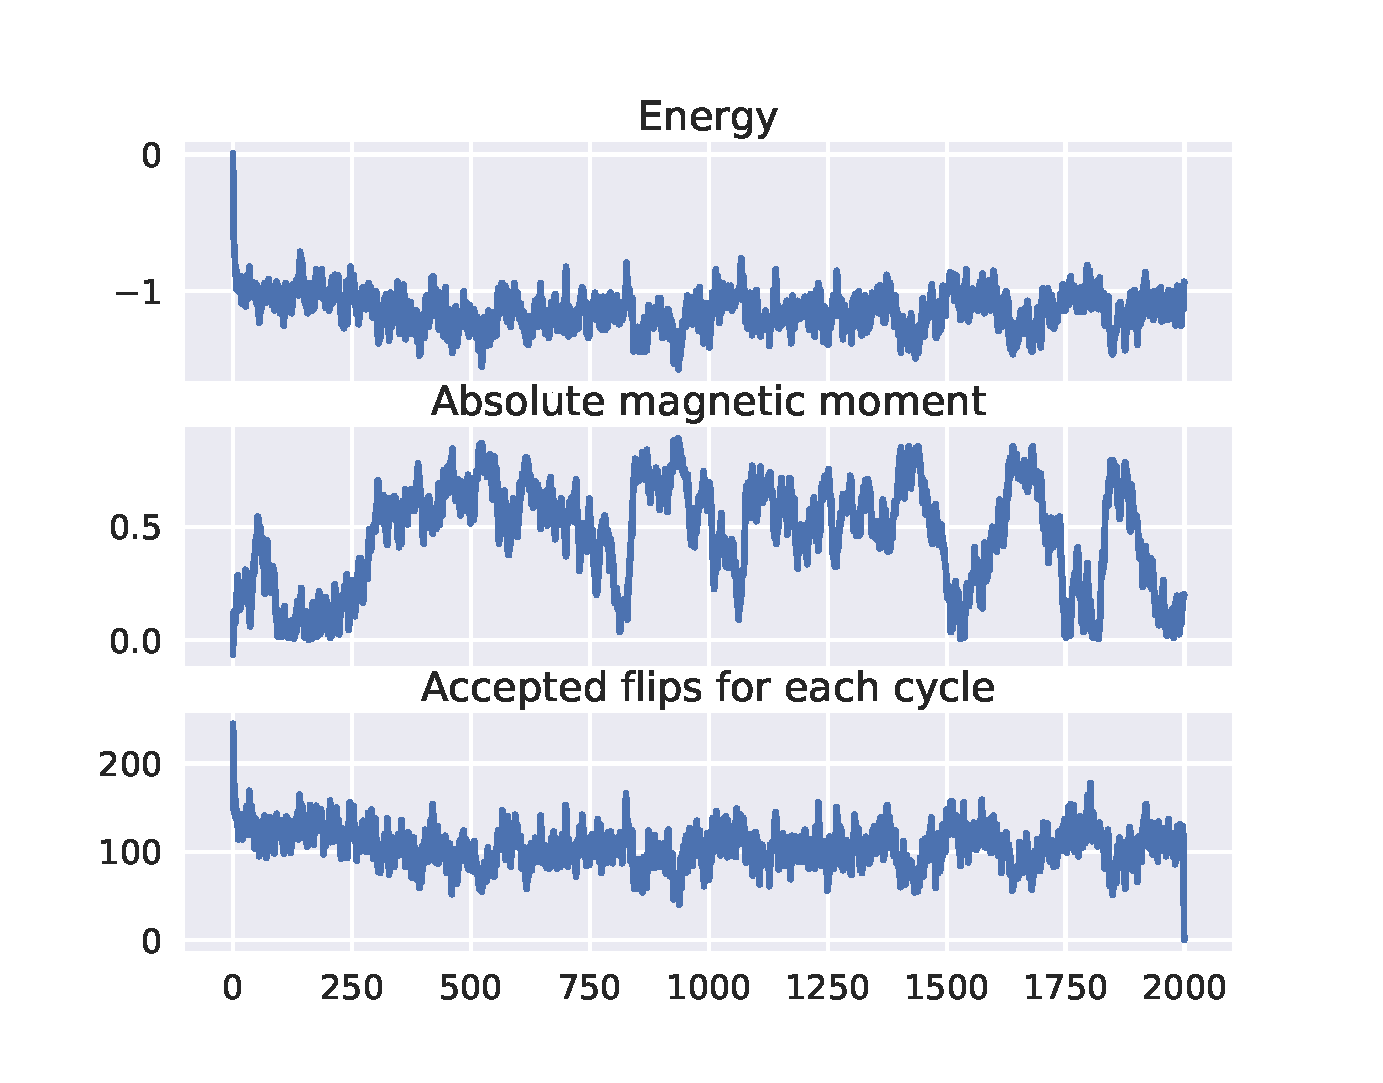
\includegraphics[width=\columnwidth]{figures/L20T2_4_random.eps}
  \caption{Energy, absolute magnetization and number of flips as a function of
  Monte Carlo cycles. The lattice size is $N = 20$, and the temperature $T = 2.4$ kT/J.
  The initial configuration is uniformly randomized.}
  \label{fig:L20T24Random}
\end{figure}
\begin{figure}
  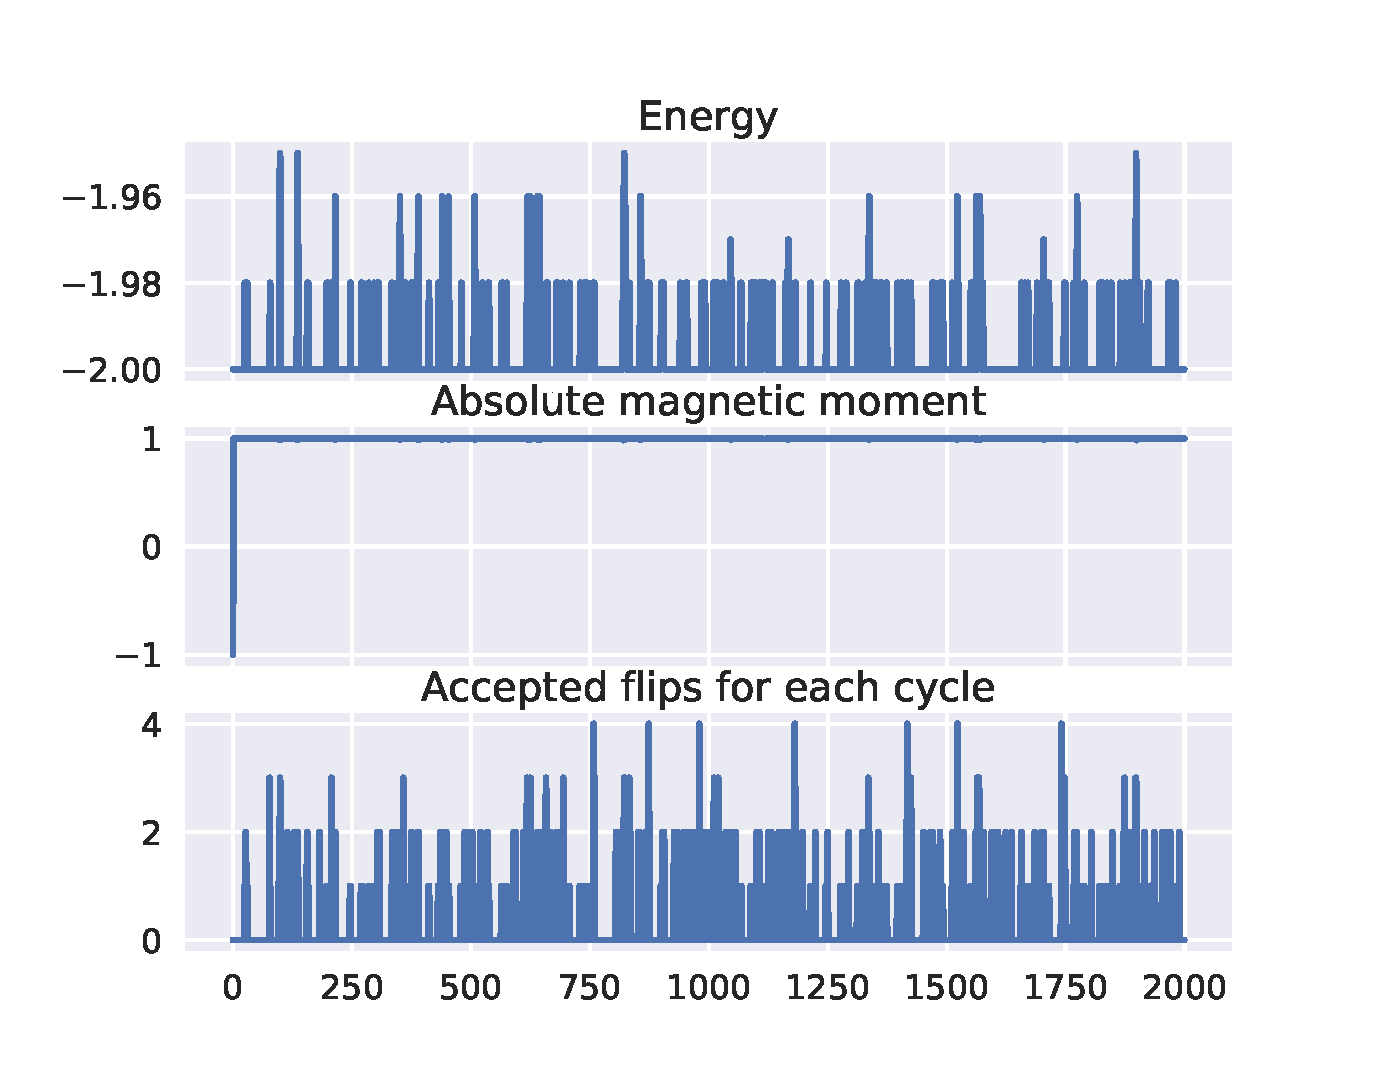
\includegraphics[width=\columnwidth]{figures/4cOrderedT1.eps}
  \caption{The lattice size is $N = 20$, and the temperature $T = 1$ kT/J.
  The initial configuration is ordered, all the spins point in the same direction.}
  \label{fig:L20T1Ordered}
\end{figure}
\begin{figure}
  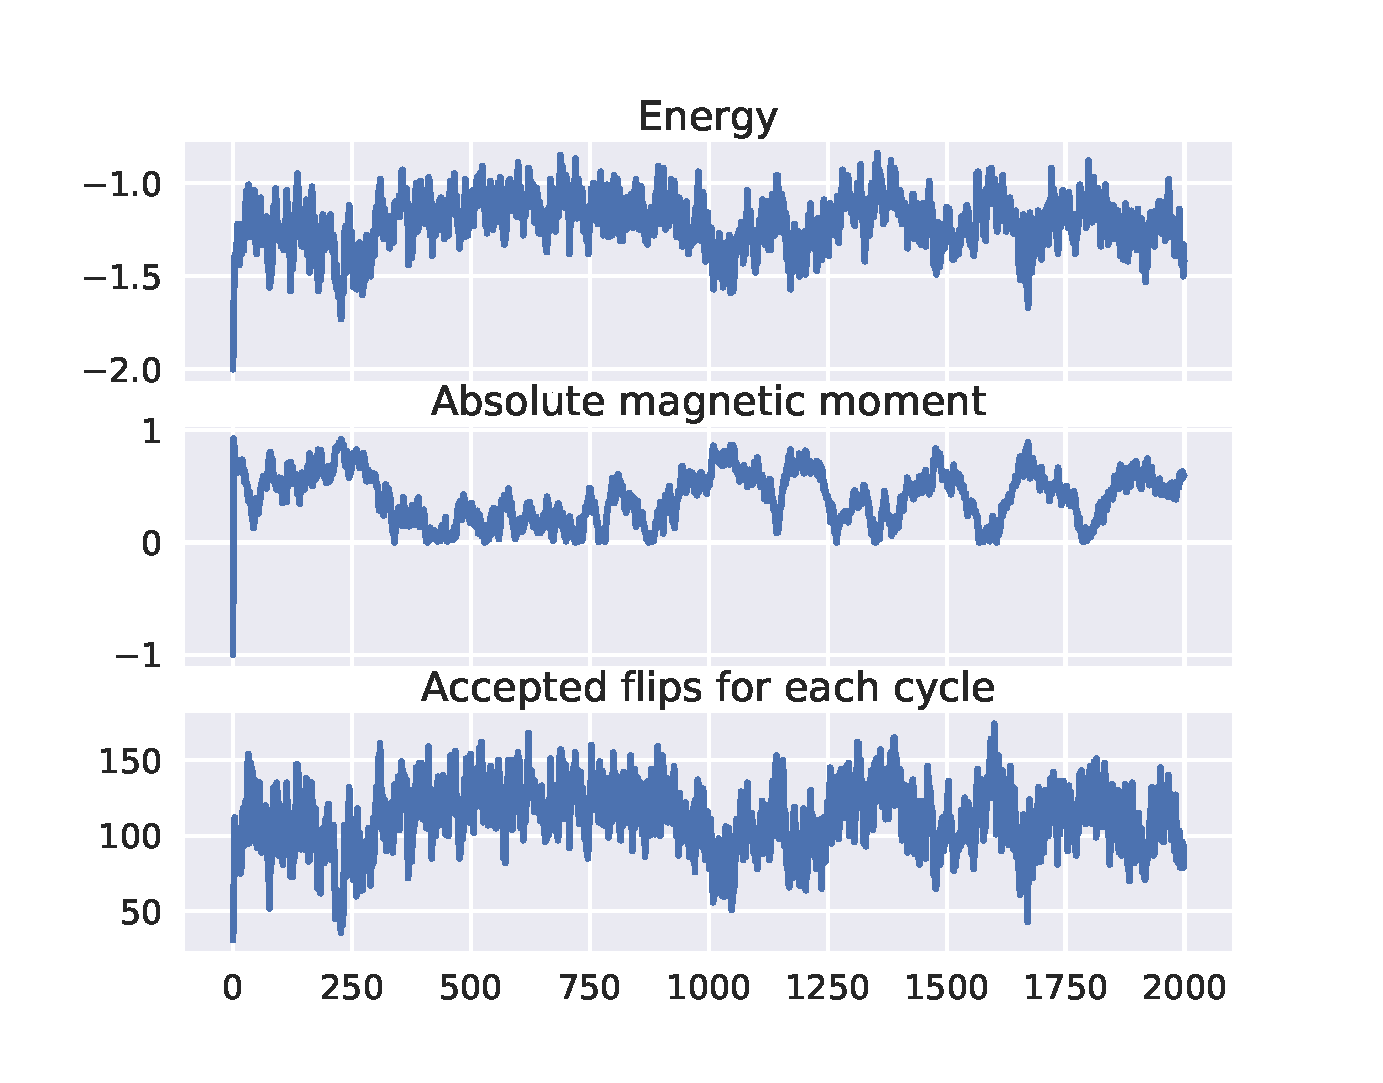
\includegraphics[width=\columnwidth]{figures/4cOrderedT24.eps}
  \caption{The lattice size is $N = 20$, and the temperature $T = 2.4$ kT/J.
  The initial configuration is ordered, all the spins point in the same direction.}
  \label{fig:L20T24Ordered}
\end{figure}
See figure~\ref{fig:4cFlips} for the total number of flips as the temperature
is increase.
\begin{figure}
  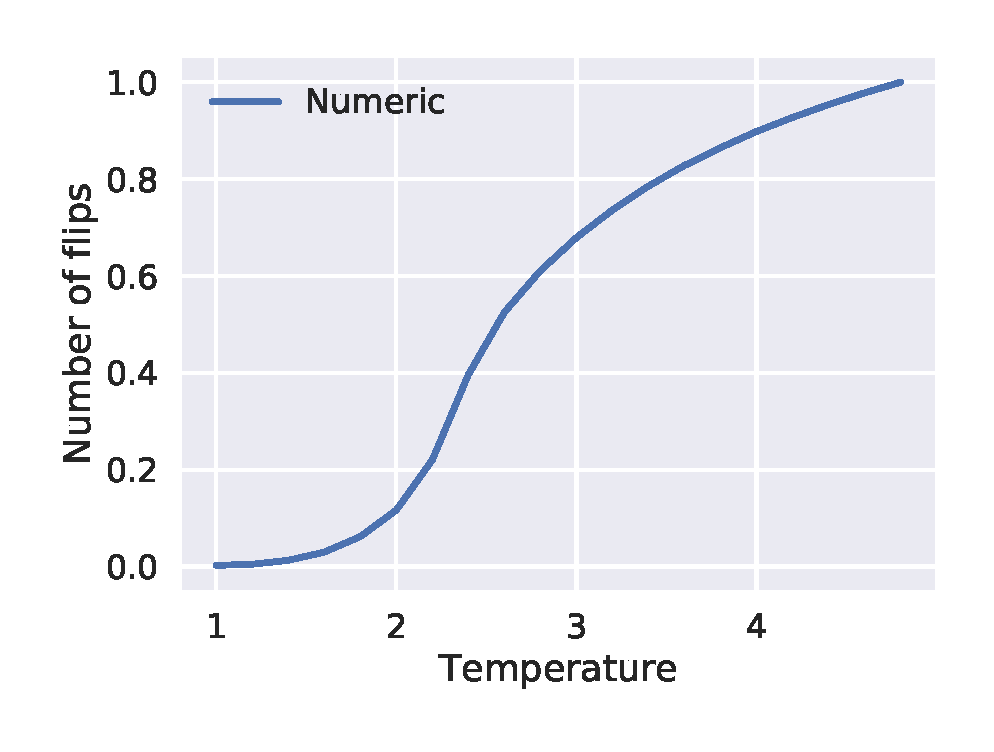
\includegraphics[width=\columnwidth]{figures/4c_number_of_flips.eps}
  \caption{Total number of accepted spin flips. The values are scaled with the
  maximum number to ease readability, and because only the temperature at which the
  slope changes is of interest. This was run with $10^5$ MC
  cycles for each temperature. Notice that the slope changes sign at around
  $T \approx 2.4$.}
  \label{fig:4cFlips}
\end{figure}

\subsection{Probability distribution}
Figures~\ref{fig:4da} and~\ref{fig:4db} show the number of occurances of energies
in certain intervals for two different temperatures.
\begin{figure}
  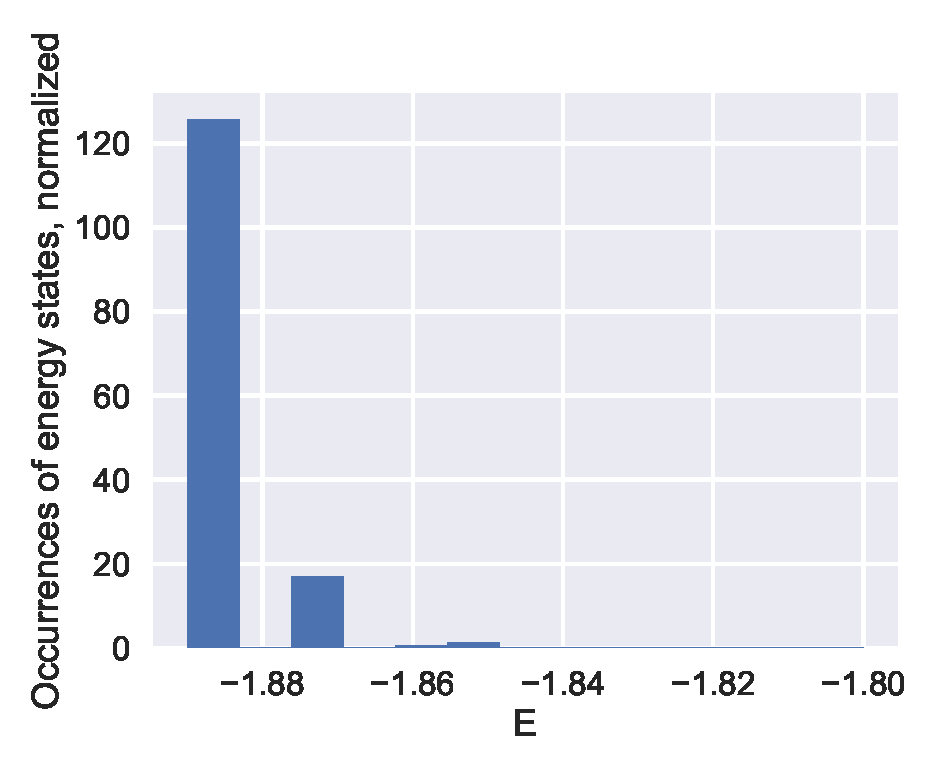
\includegraphics[width=\columnwidth]{figures/4da.eps}
  \caption{Frequency of occurances of energies in several intervals. This is
  for $T = 1$.}
  \label{fig:4da}
\end{figure}
\begin{figure}
  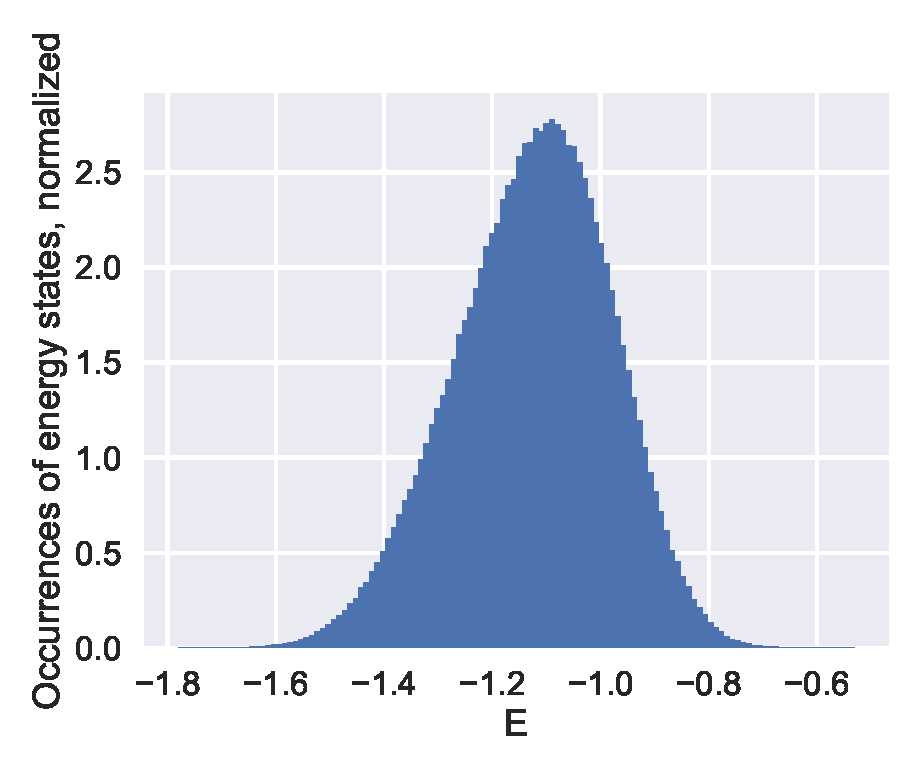
\includegraphics[width=\columnwidth]{figures/4db.eps}
  \caption{Energy frequencies for $T = 2.4$.}
  \label{fig:4db}
\end{figure}
% TODO: TA MED VARIANS AV ENERGI SOM FUNKSJON AV TEMPERATUR HER.

\subsection{Phase transition}
Figures~\ref{fig:L100Cv} and~\ref{fig:L100sus} show the heat capacity and
magnetic susceptibility as a function of temperature in the area around the analytical
value. The maximum value is found and the critical temperature is shown in the figure.
\begin{figure}
  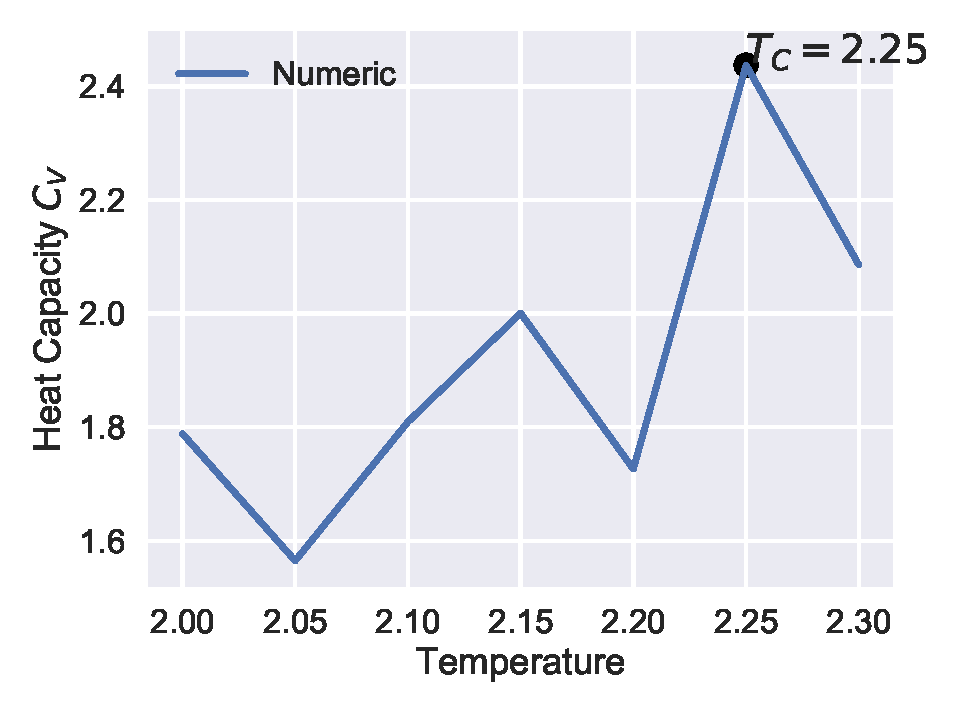
\includegraphics[width=\columnwidth]{figures/L100Cv.eps}
  \caption{Heat capacity as a function of temperature around the critical value
  for $N = 100$ as the lattice size.}
  \label{fig:L100Cv}
\end{figure}
\begin{figure}
  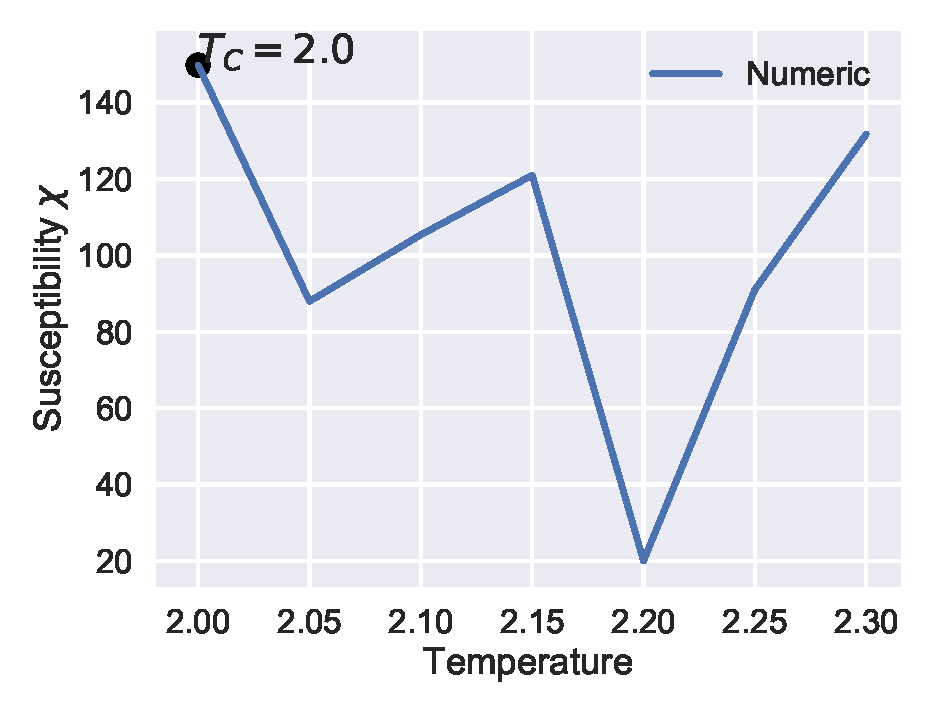
\includegraphics[width=\columnwidth]{figures/L100sus.eps}
  \caption{Magnetic susceptibility as a function of temperature, again around the
  critical temperature.}
  \label{fig:L100sus}
\end{figure}
\section{Discussion} \label{sec:discussion}
\subsection{2 x 2 lattice and analytic solution}
Figures~\ref{fig:L2Ne4},~\ref{fig:L2Ne5} and~\ref{fig:L2Ne6} show that as
the number of Monte Carlo cycles increase, the numerical solution converges to
the known analytic solution. In the latter the solutions are so similar they
completely cover each other.

As seen for the other thermodynamical quantities the Monte Carlo solution converges
to the exact solutions, at least for the $2 \times 2$ case. It is therefore reasonable
that the method should converge for larger lattice sizes, although likely slower for
larger lattices.

There is a strange linear discrepancy between the analytical and numerical
values for the energy. A similar error was seen for the expected value of the
square of the energy, which cancel out to produce correct analytical values
for the heat capacity. The source of the error is unknown, and could be either
from an incorrect analytical calculation or some error in the numerical values.
However, since the heat capacity values are correct, and the shape of the energy
expectation values are correct, the effect of the error is considered small
in terms of what the goals of this paper are.

From these results it is also possible to deduce that $M = 10^6$ should be a
decent number of cycles, although this might need to be reduced for large lattice
sizes because the simulations become very time-consuming.
\subsection{Equilibrium time}
Figures~\ref{fig:L20T1Random} and~\ref{fig:L20T24Random} show the system development
with time (actually Monte Carlo cycles, but the consideration as time has already been
explained). The first, and perhaps easy conclusion, is that an equilibrium state
seems to have been reached after around $200$ Monte Carlo cycles, at least for the
low temperature $T = 1$ and the random initial configuration. For the larger temperature of $T = 2.4$ the system has
large fluctuations around an approximately constant value, and this state is also
reached rather quickly. The higher fluctuations for larger temperature is expected,
because the Boltzmann distribution makes energy increases (exitations) more likely when the temperature
is higher.

The figure for the higher temperature also shows a very high rate and amplitude
of fluctuations for the absolute magnetic moment. This shows that for $T = 2.4$
the spins fluctuate rapidly and are aligned in the same directions for very short
time periods compared to $T = 1$, where the spins quickly go to the same direction
and remain almost constant in that configuration (almost no flips happen after
$N \approx 200$).

From figure~\ref{fig:L20T1Ordered} and~\ref{fig:L20T24Ordered} the equilibrium
time is visibly faster for the ordered initial state. For the low temperature
the initial state is the equilibrium state, and the equilibrium time is zero.
For the higher temperature, the equilibrium state is for a much higher energy,
because the spins are much more likely to flip given some d$E$ and a random
number because of the boltzmann distribution temperature dependence. The equlibrium
time for the high energy case is around the same as the low energy case, any difference
is difficult to observe from the figures.

\subsection{Probability distribution}
Figure~\ref{fig:4da} shows that only a small amount of the possible system energies occur.
This is perhaps a bit surprising, as all the states should occur statistically,
and shows that the small simulation time did not allow those small probability events to
happen. The energies at and around $-1.9$ is by far the most likely energies to be measured,
which is the energy the system converged to in figure~\ref{fig:L20T1Random}. The
bar plot essentially confirmed what was argued before, at $T = 1$ the equilibrium state
is very stable and has low variances.

For the larger temperature $T = 2.4$ (figure~\ref{fig:4db}) a much larger part of
the possible energy domain has an observable amount of occurances. This also confirms
what was argued above, the rapid fluctuations in states are naturally reflected in the
energy, which has a large variance. The mean energy is also much larger than for the lower
temperature, which also makes sense physically (A higher energy system is intuitively
more likely to be in a higher energy state).

The figure with the variance in energy further confirms the above analysis. For
larger temperatures, the system spins fluctuate more rapidly and the variance in energy
grows larger because a larger amount of energy configurations are accessed.

\subsection{Phase transitions}
The heat capacity shows a critical temperature interval that agrees with Onsagers
value. Because of the limited resolution of the simulation, it was only possible
to determine that the critical temperature $T_C \in [2.2, 2.3]$.

The magnetic susceptibility critical value does not agree with the heat capacity
or Onsager analytical values. The reason for this is unknown and rather surprising,
as the magnetic susceptibility was coherent with analytical values for the $2 \times 2$.
Although inaccurate, the value might converge to the analytical value for larger
lattice sizes, however this was not possible at this time. The result from this
figure is therefore considered inaccurate and not considered further.

The method for determining the infinite lattice critical temperature was not used
because of the lack of consistent results to compare. Despite this, for the
$N = 100$ case there is a quite good correspondance between the heat capacity
maximum and Onsager's value, which shows that the $N = 100$ lattice approximates
an infinite lattice rather well.

\section{Conclusion} \label{sec:conclusion}
The investigation of the Ising model and it's properties has shown to be a robust
model for magnetism, despite the simple nature. The $2 \times 2$ lattice
proved correct compared to analytical results and was extended to larger systems,
where analytical solutions are unavailable.

The equilibrium time was found to be lower than expected, less than $1000$ Monte Carlo cycles for the cases investigated.
The impact of initial conditions was also investigated and shown to be impactful
in terms of equilibrium time, although still quite low. The ordered initial state
provided faster convergence to equilibrium compared to the random ordering.

The probability distribution
of measuring a certain energy was also found and further showed that for larger
temperatures there is a much higher fluctuation rate for the spins.

The final part of the paper concerned phase transitions, which showed a good
correspondance with the analytical value, especially when the low amount of MC cycles
is considered. The maximum value of the heat capacity occured at $T = 2.25 \pm 0.05$, which
includes $2.269$.

A further development to the solutions and results presented here would be to
run the parallelized version on a large cluster. Although access to a cluster
was available, up to date versions of \texttt{cmake} and \texttt{jsoncpp} were not possible to install
which didn't allow for immediate runs of the program. A possible solution is to
compile \texttt{jsoncpp} or the entire code to a static library, however severe
time constraints didn't allow for this for this project. Future work on this
project would therefore ideally include such a large scale run to obtain as much
Monte-Carlo data as possible, and subsequently a more accurate estimate for the
critical temperature. The magnetic suceptibility error would also need to be
investigated and corrected.
\bibliography{references}
\blankpage
\end{document}

% Local Variables:
% TeX-engine: luatex
% End:
